\documentclass{article}
\usepackage{amsmath,amssymb,amsfonts}
\usepackage{graphicx}
\usepackage{hyperref}
\usepackage{tikz}
\usepackage{pgfplots}
\pgfplotsset{compat=1.18}

\title{Math Notes: Functions}
\begin{document}
\maketitle
Functions linear
\section{Linear and Non Linear Functions}
\section{Graphs}
\begin{figure}[h]
    \centering
    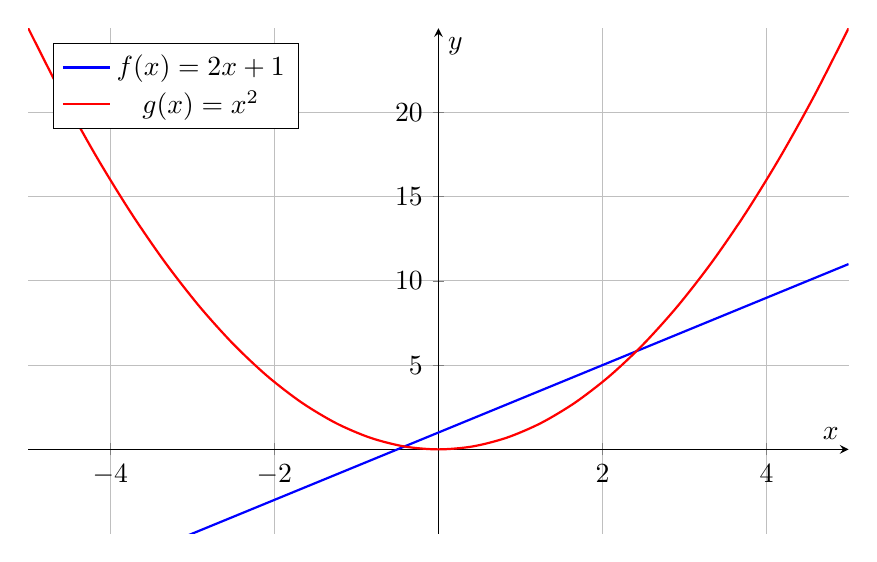
\begin{tikzpicture}
        \begin{axis}[
            axis lines = middle,
            xlabel = $x$,
            ylabel = $y$,
            xmin = -5, xmax = 5,
            ymin = -5, ymax = 25,
            xtick = {-4,-2,0,2,4},
            ytick = {0,5,10,15,20},
            legend pos = north west,
            grid = major,
            width = 12cm,
            height = 8cm,
        ]
        % Linear function: f(x) = 2x + 1
        \addplot[
            domain = -5:5,
            smooth,
            thick,
            blue,
        ] {2*x + 1};
        
        % Non-linear function: f(x) = x^2
        \addplot[
            domain = -5:5,
            smooth,
            thick,
            red,
        ] {x^2};
        
        \legend{$f(x) = 2x + 1$, $g(x) = x^2$}
        \end{axis}
    \end{tikzpicture}
    \caption{Comparison of a Linear Function $f(x) = 2x + 1$ and a Non-linear Function $g(x) = x^2$}
    \label{fig:linear-nonlinear}
\end{figure}
\section{Definitions}
Linear - going at the same pace
non linear - direction is not going at constant pace
% Important definitions go here
\section{Formulas and Equations}
% Key formulas and equations
\section{Examples}
% Worked examples or sample problems
\section{Practice Problems}
% Problems to solve or questions to answer
\end{document}
